\documentclass{article}
\usepackage{handover}


\begin{document}
\doctitle{System Overview}{Music Podcast Player}

\section{Introduction}
The Music Podcast Player is a discoverability-focused, web-based audio player built around RSS 
feeds. Artists who host their own RSS feeds can distribute music independently, without relying 
on centralized platforms like Spotify or Apple Music, allowing them to retain direct control 
over their content. Music Podcast Player fetches those feeds, then presents them in a clean, 
accessible way. This document provides a high-level overview of the system for readers 
who may be unfamiliar with the project.

\section{System Description}
Music Podcast Player lets users discover and listen to music distributed via RSS feeds. 
Users can search for feeds by keyword or input a feed URL directly. Once a feed is selected, 
its full track listing is displayed, alongside album art and artist information. Selecting 
any track begins automatic playback.

Authenticated users can organize their listening with playlists. Tracks can be added to 
existing playlists or used to create new ones. Playlists are tied to user profiles, which 
can be set to public or private and shared with others.

Music Podcast Player also supports direct artist payments through the Lightning Network. 
While a track is playing, users can send a one-time Boost, optionally including a short 
message, or enable Sat Dripping to automatically send small recurring payments at set 
intervals while they listen.

\section{Key Features}
\begin{itemize}
    \item \textbf{Desktop and Mobile Support} -- Music Podcast Player can be accessed via 
    both desktop and mobile platforms.
    \item \textbf{Keyword Searching} -- On the "Search" page, users can search the Podcast 
    Index to discover feeds.
    \item \textbf{Direct Feed Input} -- On the "Input" page, users can paste in a specific 
    feed's URL to pull up that feed.
    \item \textbf{Boostagrams} -- Users can send an artist a one-time payment, called a 
    boost, to support an artist directly. 
    \item \textbf{Sat Dripping} -- Users can enable Sat Dripping, which sends smaller 
    payments (in satoshis, a Bitcoin unit) to artists at regular intervals while listening.
    \item \textbf{User Profiles and Playlists} -- Users can create their own profile, where 
    they can create, share, and listen to custom playlists.
    \item \textbf{Modern Playback Controls} -- Music Podcast Player includes standard 
    playback controls: Play/Pause, Step Forward/Backward, Repeat Feed, Reverse Feed Order, 
    Shuffle, and Restart Song.
\end{itemize}
    
\section{Architecture Overview}
Figure \ref{fig:arch-diagram} shows the high-level architecture of Music Podcast Player. 
The frontend, built in Vue 3, communicates with a Flask/FastAPI backend, which handles 
feed fetching from the Podcast Index API, as well as user and playlist data stored in 
PostgreSQL. The entire system is hosted on AWS, with GitHub Actions managing automated 
deployment.

\begin{figure}[H]
    \centering
    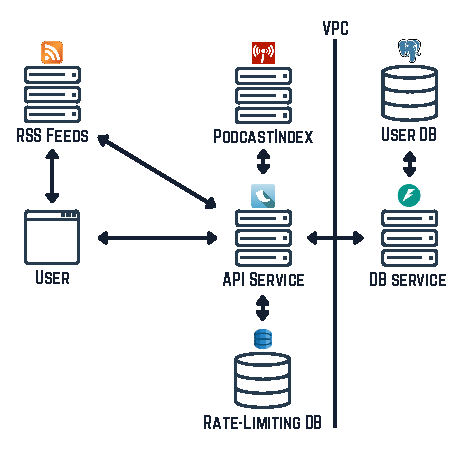
\includegraphics[width=0.5\textwidth]{architecture_diagram.pdf}
    \caption{Music Podcast Player's Architecture}
    \label{fig:arch-diagram}
\end{figure}

\section{System Boundaries and Integrations}
Music Podcast Player is responsible for feed discovery, media playback, 
user accounts, and playlist management. It does not host or store any 
audio content. Artists host their own feeds externally, and the app 
fetches and parses them on-demand via the Podcast Index API.

The system works with three external services:

\begin{itemize}
    \item \textbf{Podcast Index API} -- Feed search and discovery. 
    Music Podcast Player queries this API to retrieve feed metadata and 
    tracks.
    \item \textbf{Lightning Network} -- Handles all payment processing for 
    Boosts and Sat Dripping. Wallet authentication and transaction 
    signing are managed externally.
    \item \textbf{Amazon Web Services (AWS)} -- Hosts the application and 
    its infrastructure.
\end{itemize}

User authentication and playlist data are managed internally and stored 
in the application's PostgreSQL database.

\section{Technology Stack}
Music Podcast Player is built on a modern web stack across frontend, 
backend, data, and infrastructure layers. See Table \ref{tab:Tech Stack}.

    \begin{table}[H]
        \centering
        \begin{tabular}{l l}
            \toprule
            Category & Technology\\
            \midrule
            Frontend & Vue 3 \\
            Backend & Flask, FastAPI \\
            Database & PostgreSQL \\
            Cloud Infrastructure & Amazon Web Services (AWS) \\
            CI/CD & GitHub Actions \\
            \bottomrule
        \end{tabular}
        \caption{Tech Stack}
        \label{tab:Tech Stack}
    \end{table}

\section{Glossary}
\begin{description}[itemsep=6pt]
    \item[Boost / Boostagram] A one-time, user-defined payment sent directly 
    to an artist via the Lightning Network.
    \item[CI/CD] Continuous Integration / Continuous Deployment. A DevOps 
    practice that automates building, testing, and deploying software.
    \item[Feed URL] The direct URL pointing to an RSS feed file, used to 
    load a specific feed into Music Podcast Player.
    \item[Lightning Network] A payment protocol built on top of the Bitcoin 
    blockchain, designed for fast micropayments.
    \item[Podcast Index] An open, third-party database of podcast and music 
    RSS feeds. Music Podcast Player uses its API for feed discovery and search.
    \item[RSS Feed] (Really Simple Syndication) A standardized file format 
    that allows content creators to publish and distribute media, like 
    music or podcasts, independently, without a centralized platform.
    \item[Sat Dripping] A passive support feature that automatically sends 
    small, recurring Bitcoin micropayments to an artist at set intervals 
    during playback.
    \item[Satoshi (Sat)] The smallest unit of Bitcoin (100 million satoshis 
    = 1 BTC), used for micropayments over the Lightning Network.
\end{description}

\end{document}
